\chapter{pubertad}
En la pubertad yo estaba en estudiando en la Escuela secundaria Tecnica industrial numero 53 que esta muy serca de mi casa
a esa edad me dedique a construir tablas de multiplicar como la siguiente:
\begin{table}
	\begin{tabbing}
	\hspace*{3cm} \= \hspace*{3cm} \= \hspace*{3cm} \= \hspace*{3cm}  \kill
	\>1 \> 2 \> 3 \\
	1\> 1 \> 2 \> 3\\
	2\> 2 \> 4 \> 8\\
	.\> . \> . \> .\\
	.\> . \> . \> .\\
	\end{tabbing}
	\caption{tablas de multiplicar}
	\label{tabla_de_multiplicar.com}
\end{table}

para ayudar a unos compañeros que no les iva muy bien con las matematicas, adecir verdad fue la epoca mas divertida y buena de mi vida
porque me acuerdo que me divertia muchisimo parecia un niño como en la siguiente foto 

\begin{figure}[H]
\centering
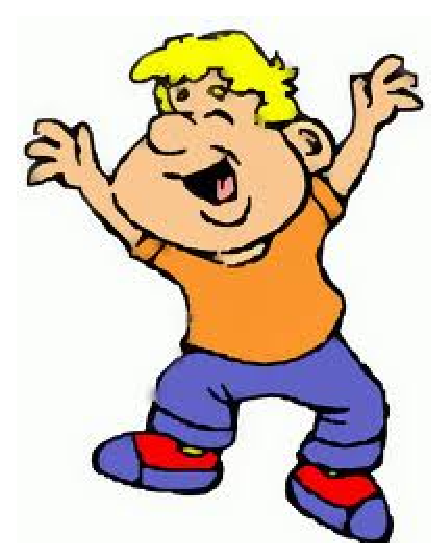
\includegraphics{fourChapter/feliz.eps}
\caption{mi pubertad}
\label{pubertad}
\end{figure}
